\chapter{Methodology}
\label{ch:Methodology}
Based on the insights from \autoref{ch:LiteratureReview}, \textit{Literature Review}, this chapter provides an overview of the key ideas and concepts needed to achieve the research objectives. The following sections will explore important concepts related to image quality assessment in teledermatology and explain the reasoning behind this work. Detailed implementation of these steps will be covered in the next chapter.\par

\section{Explorative Approach}
\label{sec:ExplorativeApproach}
\begin{figure}[ht]
    \centering
    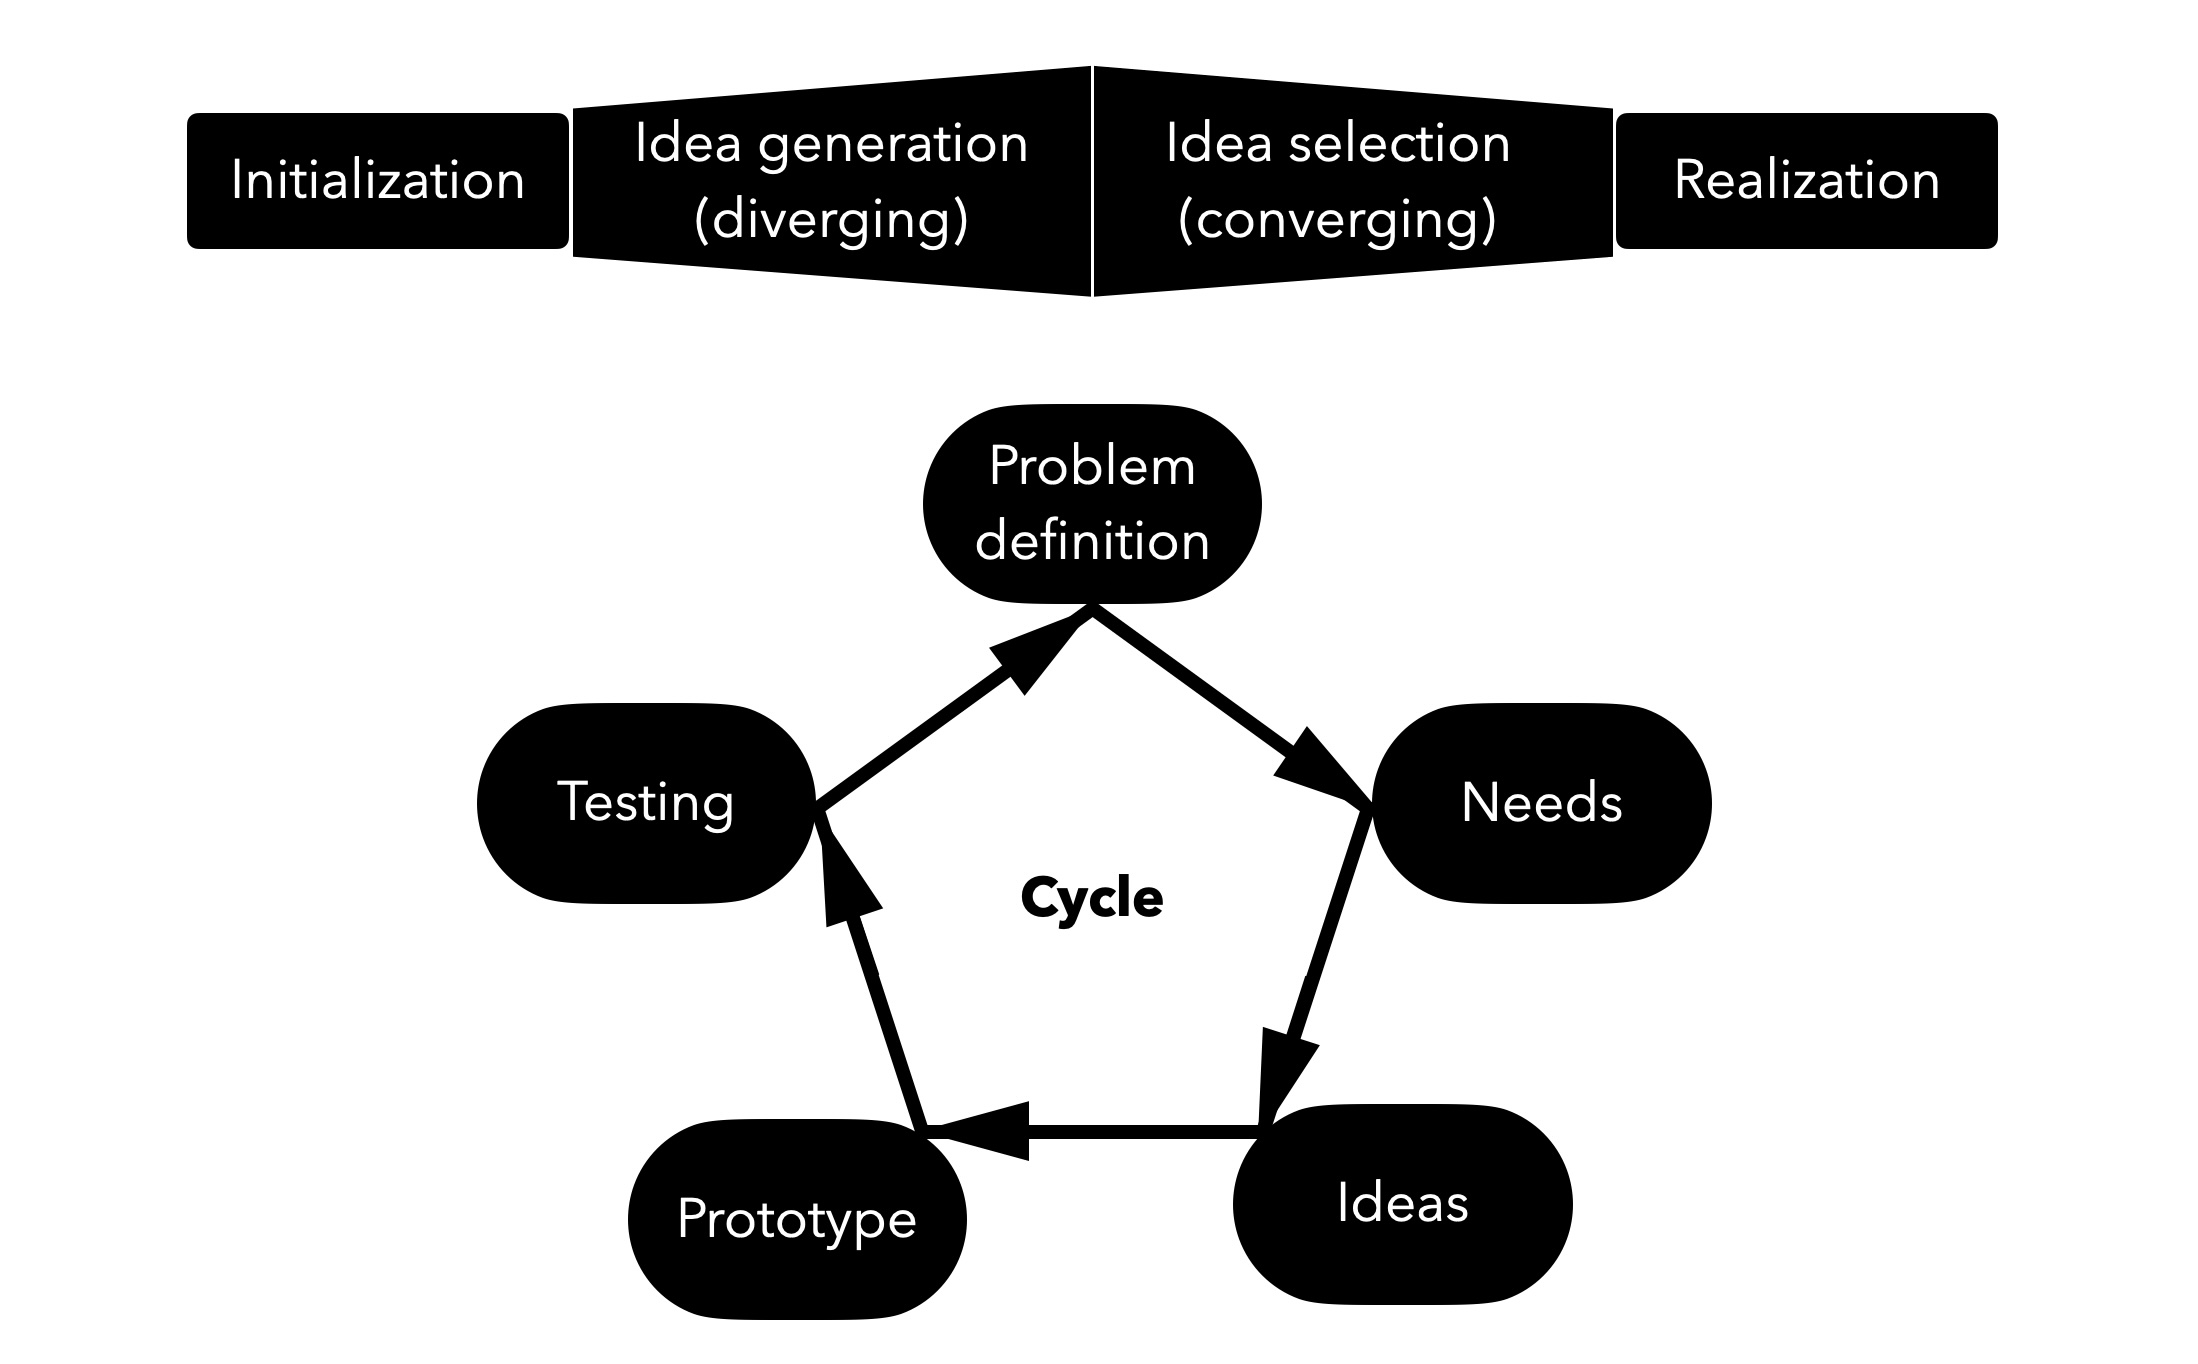
\includegraphics[keepaspectratio,width=13cm]{img/DecisionCycle.jpg}
    \caption{Visualization of the explorative approach, including the stages of initialization, idea generation, idea selection, and implementation. The lower part of the figure shows the decision cycles adapted from \autocite{DesignThinking}.}
    \label{fig:decision_cycle}
\end{figure}
\noindent
Teledermatology, especially when focused on Image Quality Assessment (IQA), offers many opportunities for innovation due to the different types of image distortions and ways to address them. To handle this complexity, an exploratory approach was used in this research. This approach is flexible and innovative, allowing for adjustments as new information is discovered, unlike traditional methods like the waterfall approach. \par
\vspace{\baselineskip}
\noindent
At the beginning, the problem was broadly defined, allowing for a flexible and adaptive approach. The research progressed through creative problem-solving with multiple learning cycles, refining ideas and methods iteratively. The project was divided into two main phases. In the \textit{Diverging Phase}, the research question’s scope was expanded to generate new ideas continuously, based on insights from the ongoing literature review. In the \textit{Converging Phase}, the focus on combining these ideas into clear findings and conclusions, aiming to create a unified understanding of the initial problem. This exploratory model is shown in \autoref{fig:decision_cycle}, which shows the stages of starting, generating ideas, selecting ideas, and implementation, along with the decision cycles \autocite{DesignThinking}.

\section{Project Control}
\label{sec:ProjectMonitoring}
Even with an exploratory approach, it is important to have a rough timeline to guide the research tasks. A workflow was established before starting, detailed in the Gantt chart attached to this thesis. \par
\vspace{\baselineskip}
\noindent
There are three key milestones identified in the first half of the project, each crucial for its success: \par
\vspace{\baselineskip}
\noindent
\textbf{Understanding Teledermatology}: Gaining a thorough understanding of the field to ensure all subsequent actions are relevant and well-informed. \par
\vspace{\baselineskip}
\noindent
\textbf{State of the Art in IQA}: Identifying the latest developments in IQA to ensure the methods used are up-to-date and effective. \par
\vspace{\baselineskip}
\noindent
\textbf{Availability of Teledermatology Data}:  Securing access to appropriate datasets for conducting meaningful IQA. \par
\vspace{\baselineskip}
\noindent
These milestones are essential because each phase of the project relies on the successful completion of the previous one. Missing any of these milestones could significantly impact the project and might require a fundamental reassessment of the objectives outlined in \autoref{sec:Objectives}. \par

\section{Research Steps}
\label{sec:ResearchSteps}
As mentioned, this study was exploratory, so it was not possible to follow a strict, step-by-step process. However, for the individual key steps, I took a systematic approach to stay organized and ensure that each step was done in the right order: \par

\subsection{Literature Review}
\label{sub:LR}
First, I began by getting an overview of my research field. As I was new to the domain of teledermatology and dermatology, this initial step was crucial. By researching and reading relevant literature, I gradually built a solid understanding of the field. Next, I identified the core topics related to my research objectives. Once I had these key topics, I carefully selected the databases to search, focusing on those most relevant to my field: PubMed\footnote{https://pubmed.ncbi.nlm.nih.gov}, Google Scholar\footnote{https://scholar.google.com}, IEEE Xplore\footnote{https://ieeexplore.ieee.org/Xplore/home.jsp}, Connected Papers\footnote{https://www.connectedpapers.com}, and Papers with Code\footnote{https://paperswithcode.com}. Using these databases, I applied search filters to narrow down the results, such as limiting the search to articles published after 2020. \par
\vspace{\baselineskip}
\noindent
I reviewed the titles of the search results and opened the ones that seemed interesting. After that, I read the abstracts to determine their relevance. Depending on the relevance of the abstract and some of the figures, I decided whether to read the full paper. Additionally, for state-of-the-art methods, I focused on finding and reading papers that had published their code and model weights if models were trained. This systematic approach ensured that my literature review was thorough and focused on the most relevant and up-to-date research. \par

\subsection{Data Collection and Preparation}
\label{sub:DataCollection}
In searching for a suitable dataset to evaluate image quality in teledermatology, a major challenge was the lack of Mean Opinion Score (MOS) or Differential Mean Opinion Score (DMOS) in teledermatology datasets, as commonly found in traditional IQA datasets mentioned in \autoref{sub:BenchmarkDatasetsIQA}. This scarcity is due to the resource-intensive nature of labeling images in the medical field. \par
\vspace{\baselineskip}
\noindent
To address this gap, I created a distortion pipeline that synthetically distorts images based on the seven criteria defined in \autoref{sub:QualityCriteriaTeledermatology}. Each type of distortion has five levels of severity, with the severity indicating how poor the image quality is. These distortions are carefully selected to simulate real-world imperfections commonly encountered in teledermatology. Each image is then labeled according to the severity and type of distortion applied, creating a dataset that not only includes the distorted images but also features precise annotations regarding their quality. This allowed me to artificially create labels for my images. For this, I needed good quality images to start with. I chose two datasets: the SCIN dataset for its relevance and uniqueness, and the Fitzpatrick17k dataset to complement the SCIN dataset. \par
\vspace{\baselineskip}
\noindent
Unlike many dermatology datasets that mainly focus on skin cancer diagnostics by classifying malignant and benign tumors, the SCIN dataset covers a broader range of common dermatological conditions, including allergic, inflammatory, and infectious diseases. These conditions are frequently encountered in everyday clinical practice but are underrepresented in existing datasets. The SCIN dataset is particularly valuable because it captures images of early-stage conditions. Over half of the images were taken less than a week from the onset of symptoms, with 30\% captured less than a day after symptoms appeared \autocite{SCIN}.  I chose this dataset because it includes conditions that patients are likely to consult about via teledermatology platforms before visiting traditional healthcare settings. The Fitzpatrick17k dataset contains more clinical setting images, which provide good quality but do not represent the variability seen in typical teledermatology images \autocite{F17K}, so I used the Fitzpatrick17k dataset only for training purposes to complement the SCIN dataset. \par 
\vspace{\baselineskip}
\noindent
In total, I selected 475 high-quality images from the Fitzpatrick17k dataset and another 475 high-quality images from the SCIN dataset for training and evaluation. Additionally, I randomly chose 200 test images from the SCIN dataset and 70 independent high-quality images from SCIN for testing. The 70 high-quality images previously selected from the SCIN dataset are fed through the distortion pipeline to introduce distortions, allowing for a consistent basis to test the model against the same types of distortions. I also labeled 200 test images, scoring each one on the seven quality criteria to ensure the model’s performance can be compared to human evaluation. \par \todo{check this subsectino again}

\subsection{Feature Extraction}
\label{sub:FeatureExtraction}
Feature extraction is the next important step where the backbone from ARNIQA is used to identify key features from the distorted images. These features capture the patterns of distortions that affect image quality. The extracted features and the generated labels are then used to train different models, including Extreme Gradient Boosting (XGBoost) regressor, XGBoost classifier, and Multi-Layer Perceptron (MLP) regressor and MLP classifier, to see which one works best for assessing image quality. \par

\subsection{Training and Validation}
\label{sub:TrainVal}
The training of the models is based on the prepared training images. Since I am generating labels and distorted images, I am not restricted by the original amount of images. I can run the images through the distortion pipeline multiple times, creating various versions of distortions from the original images. The models are then trained with these images to develop their ability to assess image quality. Validation is done in parallel with training by using a portion of the data as a validation set. This helps evaluate and monitor the performance of the models. \par 


\subsection{Testing and Experiments}
\label{sub:TestExperiment}
After completing the training, the models are evaluated using independent test data. There are two test sets used in this evaluation. The first test set consists of 70 images that were previously selected from the SCIN dataset and fed through the distortion pipeline to introduce similar distortions. This set is used to assess the actual performance and reliability of the model against consistent types of distortions. The second test set includes 200 images from the SCIN dataset, which I labeled myself, scoring each one on the seven quality criteria to ensure the model’s performance can be compared to human evaluation. \par 

\subsection{Evaluation Metrics}
\label{sub:EvaluationMetrics}
The evaluation is conducted using defined metrics such as Mean Absolute Error (MAE), R-squared (R\^2), Spearman’s Rank Order Correlation Coefficient (SRCC), and Cohen’s Kappa. The results of this evaluation provide valuable insights into the strengths and weaknesses of the image quality assessment models and serve as a basis for further improvements or adjustments. \par \todo{check this subsection again}

\begin{comment}
    	•	Mean Absolute Error (MAE): This metric measures the average magnitude of errors between the predicted and actual values, without considering their direction. It provides a straightforward indication of how close the predictions are to the actual values.
	•	R^2 (Coefficient of Determination): R^2 indicates how well the model’s predictions approximate the actual data. A value closer to 1 implies a better fit of the model to the data.
	•	Spearman’s Rank Order Correlation Coefficient (SRCC): SRCC assesses how well the relationship between two variables can be described using a monotonic function. It is useful for measuring the strength and direction of the association between the predicted and actual image quality scores.
	•	Cohen’s Kappa: This statistic measures inter-rater agreement for categorical items, indicating how much better the model’s predictions agree with the actual labels compared to chance. It is particularly useful for evaluating classification models.

By using these metrics, the performance of the image quality assessment models can be comprehensively evaluated, providing insights into their accuracy, reliability, and overall effectiveness in assessing image quality in teledermatology.
\end{comment}

\subsection{Discussion and Further Development}
\label{sub:DiscussionDevelopment}
In conclusion, the results of the project are analyzed and discussed. This discussion includes an evaluation of the achieved goals, an analysis of the challenges and limitations of the project, and a look at possible further developments. Additionally, potential applications of the developed image quality assessment models in teledermatology are considered, along with the opportunities and challenges that arise from these applications. \par